
%%% Local Variables: 
%%% mode: latex
%%% TeX-master: t
%%% End: 

\chapter{命名服务网络设计}
在\ref{SCN-intro}中介绍了集中以信息中心网络为基础的服务网络设计,以上设计方向主要分为两类:
\begin{itemize}
\item 利用服务来对网络连接进行抽象以提高在网络层面的网络服务质量:典型的如SOFIA\cite{wu2014sofia}网络,将命名数据包进一步抽象成命名服务包并对服务转发进行控制。而SERVAL\cite{nordstrom2012serval}网络中,虽然不是直接以ICN为原型,但是通过服务名对数据包进行抽象以达到对网络流量更好的控制。
\item 另一种通过对服务进行抽象以实现功能性网络:典型的如Service Centric Networking\cite{braun2011service}中,通过将数据请求重新封装为服务命令请求,以实现远程调用。在Named Function Networking\cite{tschudin2014named}中不仅以数据处理为核心定义了数据处理请求,同时重新设计了NFD的流程,添加了主动的数据处理整合表达式($\lambda$表达式)。
\end{itemize}

本文旨在通过基于ICN的性质,在网络层面集成网络服务功能,来探索在命名数据基础上进行服务抽象的网络的新的特性。W3C的web service标准参考了WSMF的模型,WSMF模型同样需要基于一些基本要素包括:文档类型,语义,相关传输协议,信息交换序列,流程,安全,句法以及服务配置。文章\cite{pautasso2008restful}中提供了一套比较RESTful Service与Web Service的框架。该框架更加详细地分析了两种web服务在架构设计方面的选择原因。在以往的研究中基于信心中心网络的服务首先没有对服务的前提条件进行研究,同时也没有一套对于服务的基本建模。本节旨在首先结合现有的服务分析框架提出在ICN之上做服务网络的架构选择,提出服务模型,并总结一套设计原则。基于该服务模型,开发命名服务网络原型并进行实验评估。

\section{命名服务网络设计原则}
在第\ref{repo}章中,介绍了NDN Repo协议。本文提出的命名服务网络(Named Service Networking,NSN)以NDN Repo协议设计为蓝本来进行设计。本节采用文献\cite{pautasso2008restful}中的分析框架,对命名服务网络架构在设计上的选择进行分析。

\subsection{设计原则比较}
基于NDN Repo协议以及repo-ng的实现,同Restful Service与Web Service在架构原则上进行比较。

Rest架构利用HTTP动词作为接口的动词,将HTTP协议作为应用的一部分。而WS-*的SOAP协议中HTTP只是Web Service的文档传输协议。Repo协议的实现过程中,采用了类似于Rest的实现方式,将服务请求的语义与NDN的interest结合,即在interest的请求中封装服务请求参数。

Restful Web架构为典型的客户端服务器架构,通过HTTP协议将客户端,浏览器,服务器等连接起来。Rest的异构性通常来自不同的浏览器生产商对HTTP协议的解析渲染的不同。SOAP和WS-*起源于异构性更强更加服务的自治域,甚至可以集成Web出现之前典型的COBOL程序,或者COBRA架构的系统。在WSMF模型中,一个服务的基本要素为:文档类型,语义,传输协议,信息交换序列,流程,安全,句法,服务配置,这8个元素都可以造成客户端与服务端或者服务端之间产生异构性。NSN架构需要解决的第一个主要问题就是\textbf{基本服务要素之间的异构性}。

在松耦合方面,无论是Rest,WS-*以及NSN都与地点解耦。WS-*架构同时具备高可用性,在网络中断或者服务端宕机时,WS-*客户端可以将请求放进队列。而REST架构为远程RPC模式,更倾向为同步调用。在Repo协议中,无论是插入还是删除流程,都定义了在插入不成功的情况下,重传,或者遇到错误返回的情况,更加倾向于RPC模式。但是在repo-ng的具体实现过程中,客户端可以在本地实现队列结构,未被满足的请求可以定期的进行重试。

在服务扩展方面,NSN采用了TLV格式,为典型的树桩结构文档,可以对服务功能进行扩展。


\begin{table}[h]
\centering
\caption{设计原则比较}
\label{tab:arc-principle-comparison}
\begin{tabular}{l|lll}
架构设计原则 & REST & WS-* & NSN \\ \hline \hline
协议层次 & yes & yes & yes \\ \hline
HTTP作为应用层协议 & \checkmark &  &  \\
HTTP作为下层传输协议 &  & \checkmark &  \\
NDN作为应用传输协议 &  &  & \checkmark \\ \hline \hline
异构性处理 & yes & yes & yes \\ \hline
浏览器之间 & \checkmark &  &  \\
企业级中间件 &  & \checkmark &  \\
需要研究 &  &  & ? \\ \hline \hline
松耦合 & yes & yes & yes \\ \hline
可用性(时间) &  & \checkmark & ? \\
位置 & \checkmark & \checkmark & \checkmark \\
服务扩展: &  &  &  \\
统一接口 & \checkmark &  &  \\
XML可扩展 & \checkmark &\checkmark  &  \\
TLV可扩展 &  &  & \checkmark \\ \hline \hline
\end{tabular}
\end{table}

\subsection{概念比较}

WS-*有远程调用以及消息集成两种方式。\cite{vinoski2002putting}而消息集成的方式更加适合松耦合系统的集成。在Repo Protocol中,采用的是远程调用(RPC)的集成方式。在NSN设计,需要定义的第二个问题是\textbf{如何以消息形式集成异构系统}。

在WS-*实现过程中,WSDL作为对服务的描述,另一方面可以看做服务的契约(contract)。在WS-*实现中,有contract-first和contract-last两种方式。REST架构没有一种描述文档,所以为contract-less。在Repo协议以及NDN packet specification中,对TLV文档有描述文档,可以在TLV描述文档基础上定义类似于WSDL的NSN服务描述文档。

Restful架构本质上是对URI所代表的资源进行状态转移。而WS-*是面向服务对象。在Repo协议中,利用URI名字的前缀代表需要操作的对象,通过URI后面封装的文档来对服务进行操作,是一种介于Rest和WS-*之间的模式。

同Restful架构一样,NSN架构需要对资源描述URI设计采用一种漂亮的方法。需要保证URI的持久性,简洁性,可读性,具体化(倾向使用名词),一致性以及抽象性(不要暴漏实现细节)。

在NDN协议中,数据采用TLV的格式进行封装。在NDN repo协议中,定义了一套描述协议报文格式的TLV描述。该描述虽然定义了请求的基本语义,但是没有一套类似于WSDL对于请求响应过程等描述。在NSN设计中,需要定义的第三个问题为\textbf{如何对NSN服务进行描述}。

\begin{table}[h]
\centering
\caption{概念比较}
\label{tab:arc-conceptual-comparison}
\begin{tabular}{l|lll}
架构设计概念 & REST & WS-* & NSN \\ \hline \hline
集成方式 & 1AA & 2AAs & ?AA \\ \hline
远程调用(RPC) & \checkmark  & \checkmark & \checkmark \\
消息 &  & \checkmark & ? \\ \hline \hline
契约设计 & 1AA & 2AAs & ?AA \\ \hline
Contract-first &  & \checkmark & ? \\
Contract-last &  & \checkmark & ? \\
Contract-less & \checkmark &  & ? \\ \hline \hline
服务标注 & 1AA & n/a & ?AA \\ \hline
自己实现 & \checkmark &  & ? \\ \hline \hline
URI设计 & 2AAs & n/a & 2AAs \\ \hline
“Nice” URI scheme & \checkmark  &  & \checkmark \\
No URI scheme & \checkmark &  & \checkmark \\ \hline \hline
数据表述方式 & yes & yes & yes \\ \hline
XML schema &  & \checkmark & ? \\
TLV schema &  & & \checkmark \\
自定义 & \checkmark &  & \\ \hline \hline
\end{tabular}
\end{table}

\subsection{技术比较}
本节讨论在服务网络实现中,在安全性,可靠性,服务集成以及服务发现的架构选择。

\begin{table}[h]
\centering
\caption{技术比较}
\label{tab:arc-tech-comparison}
\begin{tabular}{l|lll}
架构选择 & REST & WS-* & NSN \\ \hline \hline
安全 & 1AA & 1AA & 1AA \\ \hline
WS-Security &  & \checkmark & \\
HTTPS & \checkmark &  & \\
NDN-Security &  &  & \checkmark \\ \hline \hline
传输可靠性 & 1AA & 4AAs & ?AA \\ \hline
HTTPR & (\checkmark)  & (\checkmark) & \\
WS-Reliability &   & \checkmark & \\
WS-ReliableMessaging &   & \checkmark &  \\
Naive &  & \checkmark &  \\
自定义 &  & \checkmark & ? \\ \hline \hline
服务集成 & 2AAs & 2AAs & ?AA \\ \hline
WS-AT &  & \checkmark & ? \\
自定义 & \checkmark & \checkmark & ? \\ \hline \hline
服务集成 & 2AAs & 2AAs & ?AA \\ \hline
BPEL &  & \checkmark & ? \\
Mashups & \checkmark &  & ? \\
自定义 & \checkmark & \checkmark & ? \\ \hline \hline
服务发现 & 1AA & 1AA & ?AA \\ \hline
UDDI &  & \checkmark & ? \\
自己实现 & \checkmark &  & ? \\ \hline \hline
\end{tabular}
\end{table}

WS-*的服务安全采用WS-Security协议\cite{atkinson2002web},而REST安全通常是基于HTTPS提供信任保证。HTTPS的安全模型相对简单,提供的只是点对点的加密以及签名,无法解决跨信任域的安全策略以及信任模型。WS-Security利用现有的相对成熟安全标准与规范来实现,利用X.509和Kerberos进行签名以及身份验证,密钥管理可以基于KPI。由于SOAP协议是基于XML文档进行传输的,采用对XML文档进行加密或签名,在XML的子文档头中封装签名信息。NDN的安全策略与WS-Security类似采用基于文档的安全方式,证书信息封装在NDN命名数据包中。NDN没有指定特定的安全模型,安全策略与信任模型的设计同数据安全通道设计分离。NSN在NDN的基础上采用interest与data双向的安全通道策略。

在WS与REST的工业实现中,数据的可靠传输依靠TCP或TCP类似的可靠传输协议。RESTful作为一种服务实现风格,没有HTTP之上的可靠传输处理流程。WS-*目前有WS-ReliableMessaging\cite{ferris2005web}和WS-Reliability\cite{iwasa2004ws}两种标准。架构基本思路为通过将不可靠基础设施的服务消息传输借道可靠传输通道。在Repo协议中,可以看到对于传输的控制只是对传输正确性的控制,而不是对报文可靠传输真正的控制。NDN并没有对通信有可靠传输保证,NACK也并没有加入到现在的NDN协议之中。作为NSN的扩展,NSN设计的第四个问题为\textbf{如何进行可靠传输协议设计}。

在传输可靠性基础之上就是服务可靠性,即对事务的支持。在WS中提供了对于原子性事务的支持WS-AT。对于分布式事务的支持即为服务集成的基础。

在服务集成上,REST架构没有一个统一集成的标准,在某些领域有通过REST通信方式集成资源的专门协议,如OAuth来解决第三方网站之间信任与认证的问题\cite{hardt2012oauth}。对于Web Service服务集成的研究相对比较成熟,最典型的以BPEL为基础的服务流程集成系统。NSN系统如果想进行功能可扩展同样需要对服务集成的支持。NSN设计的第五个问题为\textbf{如何设计NSN服务描述以支持服务集成},其中包括对于事务扩展以及集成状态触发的支持。

\section{命名服务网络协议概述}
在\cite{braun2013service}中,提出了一种基于ICN的服务网络架构,包括服务解析,服务参数与类型支持等。然而,仅仅拥有这些因素还是无法构建一个分布可用的服务网络。在\cite{fensel2002web}中,提出了一种基于Web Service的服务模型。WSMF模型在\ref{WSMF-arc}中已经进行了介绍,指出了一个可用服务的要素,包括文档类型,语义,传输协议,信息交换序列,流程,安全,语法以及服务配置。

\textbf{服务描述}机制并没有在SCN中阐述。\cite{braun2013service}尽管在SCN中服务请求可以封装命令及相关参数,但在没有服务描述的情况下,客户端与服务端的设计无法做到松耦合。在Web Service中,WSDL用来让web应用去“懂得”如何调用某服务。

\textbf{服务发现}在大型可扩展的网络同样必不可少。Web Service中通过UDDI来管理服务描述文档,并对服务进行简要描述。同样在Web Service基础上有一些街自动服务发现的相关研究。\cite{klusch2006automated,schmidt2004peer,schlosser2002scalable}

\textbf{服务协调}意义在于协调不同的服务语义使服务之间能够以更加可扩展的方式进行沟通。在服务升级过程中,服务语义之间会发生不同版本共存的情况。语义网的本体论技术可以在不同语境下去融合不同的语义术语。

在\cite{braun2011service, braun2013service}中,提出的基于CCN网络的SCN框架可以归纳如下:

\begin{enumerate}[a]
\item 命名:利用$\left\langle content\_owner, content\_name\right\rangle $的命名结构来整合结构化与扁平化命名
\item 服务解析:服务名字与服务地址的匹配
\item 服务参数:在服务与网络耦合的网络中,修改各种ICN网络中内容请求的格式,将请求服务参数放置于内容请求中,如CCN网络;在服务与网络解耦的设计中丰富服务描述系统,如PURSUIT网络
\item 服务部署:通过向服务开发者提供网络环境参数,以优化服务部署方案
\end{enumerate}

但是上面a - d四点无法提供基于ICN的可扩展服务。基于Web Service中的WSMF模型\cite{fensel2002web},提出基于NDN的NSN设计的基本原则:

\begin{enumerate}[a]
\item 在NDN基础上的应用层进行服务网络设计
\item 修改服务请求使服务请求可以被安全验证
\item 可扩展的服务语义与服务描述
\item 建立可扩展的服务解析与发现系统
\item 相似语义的服务可以被协调
\end{enumerate}

基于NDN网络的NSN概念设计如图\ref{fig:NSN-arc}所示,对于NDN网络,NSN层面需要在NDN层面上进行定制化的改动,例如修改Interest名字的结构。

\begin{figure}[H]
  \centering
  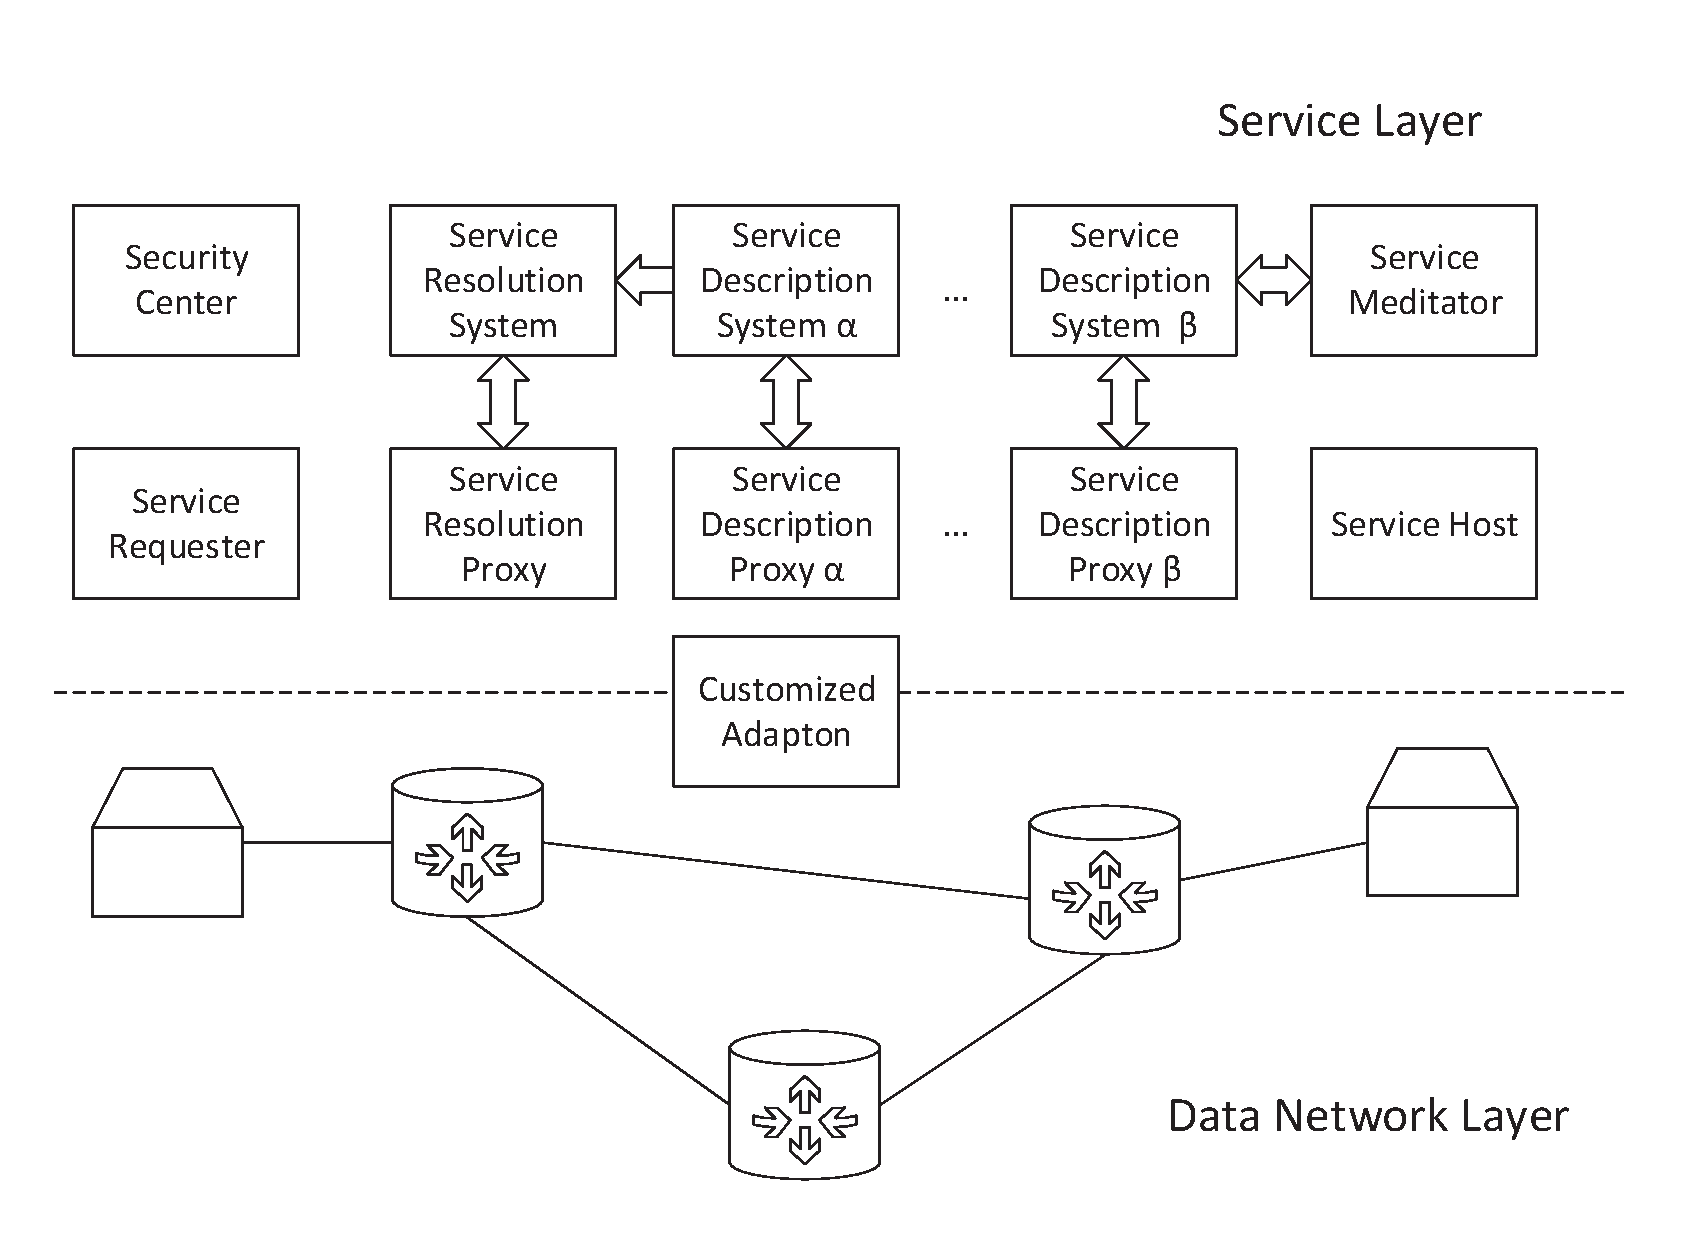
\includegraphics[width=0.8\textwidth]{NSN-ICN}
  \caption{NSN概念架构设计}
  \label{fig:NSN-arc}
\end{figure}

\subsection{服务抽象}
在ICN网络中,网络的作用对命名数据请求响应对应的命名数据。在命名服务网络(NSN)中,网络的目的是用来传输指定的命名服务请求,对该请求进行响应处理并对服务请求者返回请求结果。NSN利用NDN作为下层数据传输协议,采用类似于RESTful方式,将服务请求封装在NDN数据请求之中,NDN数据包封装服务响应。NSN并没有修改下层NDN协议,包括网络包封装协议,路由协议等。NSN可以被看做基于NDN的一种分布式应用服务。在NSN中,服务请求是服务的触发条件,服务的标识为服务的名字,采用NDN URI的命名惯例。服务描述以TLV描述文档为基础,构建类WSDL的文档描述协议。

\subsection{安全}
安全性为服务网络可用性的基础。服务安全性最基础的要求为,服务请求与响应可被验证与加密。除此之外需要服务请求与响应所绑定的安全身份可以被公开验证。服务请求所绑定的安全身份可以被用来进行服务访问控制。

NDN采用基于内容/文档的安全机制。所有的数据包采用密钥进行数字签名,证书信息被封装在数据包之中。在原始的NDN协议中,并没有对数据请求签名的支持。在NSN中,采用在NDN静态库ndn-cxx中SignedInterest\footnote{Signed Interest: http://named-data.net/doc/ndn-cxx/0.3.1/tutorials/signed-interest.html}的实现。

NSN的双向签名网络包是实现安全的基本保证。在NSN设计中,上层具体的安全构建并没有作为强制标准,在NSN实现中采用安全中心设计。在当前的签名与加密实现中,工业界普遍采用对称/非对称密钥方式,如Kerberos或X.509。在对称密钥体系如Kerberos中,需要Kerberos认证服务器(AS)作为证书管理与信任锚点(trust anchor)。在非对称密钥体系中,需要公钥基础设施(PKI)对证书与密钥进行管理,需要trust anchor对于证书身份进行验证。无论是何种安全体系,都需要一个相对集中的安全管理角色。在NSN架构实现中,该角色为安全中心。NSN安全中心不是特指具体某一个主机,可以为架构或p2p层次的主机群。

\subsection{服务解析}
在SCN中,服务解析指的是服务寻址。对于通过服务一般描述来获取服务描述文档,单纯的名字寻址无法满足要求。当前通过服务描述来获得具体服务文档的话有如下几种方式:

本体论:例如在语义网实现的Web Service实现中,OWLS-MX提供了一种基于本体论的具有语义推导功能的服务发现协议。\cite{klusch2006automated}

分布式查询系统:分布式查询系统可以将服务发现服务进行分布式布置,利于系统服务的扩展。典型系统如基于本题论的Hypercube P2P系统\cite{schlosser2002scalable},以及基于分布式哈希的关键词查询系统\cite{schmidt2004peer}。

WS-*工业一般实现中采用UDDI的集中式注册目录作为服务发现系统。在NSN设计中,采用服务解析代理作为服务请求者服务解析入口。NSN服务解析层次作为独立的系统接收服务解析代理的查询请求。在实际系统实现中,NSN采用关键词搜索方案。当前互联网解析服务中,本体论应用场景比较少。随着搜索引擎技术的发展,关键词匹配的技术效果越来越好,同时采用关键词方法的学习成本相对较小。同时有一些方便的开源项目例如Apache Lucene\footnote{Apache Lucene: https://lucene.apache.org/core/}提供了非常方便的文档关键词查询的解决方案。

服务解析代理需要预先定义好服务解析的语义,并了解服务解析主机的名字。服务解析代理只是负责发送服务解析请求,并需要了解服务解析主机服务的部署方式,无论是中心化,层次化还是P2P的。

\subsection{服务描述}
\label{description}
对于一个服务描述需要包含以下六个元素:
\begin{enumerate}[a]
\item 服务的名字
\item 服务描述与关键词:用来在文本上描述服务,并为服务发现提供索引依据。
\item 功能列表:该服务可以提供功能的名字列表
\item 先决条件(Pre-condtions):触发服务某功能需要的先决条件,通常情况下为输入参数。此外,对于支持状态的服务,同样包含触发服务需要的状态。
\item 输出条件(Post-conditions):描述在不同状态下服务的返回条件。通常为返回值参数描述。在状态服务下,同样会输出服务状态的变化。
\item 服务拥有者。
\end{enumerate}

一个典型的服务描述如下所示,该服务描述描述了一种数据存储服务。该服务基本功能参照NDN Repo协议,通过普通的NDN interest来获取数据,数据插入与删除作为服务功能开放。该描述用伪代码部分展示如后框图所示。WSDL中,对于服务的描述以XML形式进行封装。虽然在概念设计上,NSN服务描述没有规定指定的文档格式。在实现中则采用TLV结构的可扩展的文档结构。服务代理当有服务的确切名字时,可以利用该名字发送interest,请求服务描述数据包。服务描述系统将服务描述数据包返回给服务代理。而根据关键词以及部分文档描述进行查询则被当做服务描述系统的一种服务对外开放,接收的是服务请求而不是单纯的数据请求。

Web Service中WSDL设计的要素包括:definitions,types,portType,operation,binding,service以及port。在NSN中,由于专门binding在NDN上,operation可以作为名字的一部分封装在服务请求中,并与服务描述中的function list的名字进行一一对应。此外在TLV文档描述中,描述了输入参数的类型,对应于WSDL中的Type。WSDL中definitions即作用域可以用名字的前缀来进行对应。在形式上WSDL与NSN的文档描述可以进行等价。

\begin{figure}[h]
\begin{framed}
\begin{verbatim}
Repo Service Description

Name: /THU/repo
Description: insertion and deletion of data packets
Keywords: repository, repo, insertion, deletion, removal,
          data packet
Function List:
    Name: insert
        Description: put data packets into repo
    Name: delete
        Description: remove data packets from repo
PreCondition:
    FunctionName: insert
        Parameter: DataName
            DataName: BYTE
    FunctionName: delete
        Parameter: DataName
            DataName: BYTE
PostCondition:
    FunctionName: insert
        Result: StatusCode
        StatusCode: INTEGER
    FunctionName: delete
        Result: StatusCode
\end{verbatim}
\end{framed}
\end{figure}

\subsection{服务协调与集成}
在前述服务描述文档结构中,为服务集成提供了输入与输出状态描述。在Web Service服务集成中,分别有Orchestration和Choreography两种模式。考虑到NSN对于服务的描述与WSDL在形式上可以进行等价。对于BPEL的设计经验同样可以移植在设计NSN的服务集成当中。

除了服务集成之外,还有就是语义协调。文档的设计上可以分为兼容关系与匹配关系两种,对于服务描述文档的兼容或匹配的判断可以交给NSN中专门的协调单元。

在图\ref{fig:NSN-arc}中,mediation模块抽象的代表了服务集成引擎(类比于BPEL engine)以及服务语义协调的功能。

\section{命名服务网络原型实现}
命名服务网络NSN原型基于NDN的开源代码库,包括ndn-cxx,NFD以及NLSR。通过修改ndn-cxx基础库,增加对于NSN服务描述的支持。NSN原型实现了三种服务,包括空服务,即服务端只返回一个空内容的服务返回包;基于NDN Repo协议的存储服务;提供简单四则运算的计算服务。本节将分别介绍各个要素的实现。原型实现代码已经在Github上开源:https://github.com/chenatu/repo-service

\subsection{命名}
服务请求的命名方式采用NDN的模块化URL。在当前的NDN网络包中,采用TLV的封装格式,TLV可以通过子模块组合而成。在NDN命名中,数据请求的名字为完整的TLV模块,通过每个子名字单元TLV模块组合而成。而每个子单元可以由更加小的TLV模块组合而成,由此可以封装服务请求的参数。服务请求的名字结构如下所示:
\begin{framed}
\begin{verbatim}
/service name/function name/parameter
\end{verbatim}
\end{framed}
其中function name模块为服务描述function list中服务功能名字。parameter结构可以对参数进行结构化封装。以数据插入请求为例,参数的TLV结构为:
\begin{framed}
\begin{verbatim}
Parameter ::= REPOCOMMANDPARAMETER-TYPE TLV-LENGTH
                           Name?
                           Selectors?
                           StartBlockId?
                           EndBlockId?
                           ProcessId?
                           MaxInterestNum?
                           WatchTimeout?
                           WatchStatus?
                           InterestLifetime?
\end{verbatim}
\end{framed}

其中Parameter可以由包括Name,Selectors在内的子结构组成。

\subsection{安全}
NSN的安全设计采用NDN Repo协议中的基本安全设计。采用Signed Interest与Signed Data Packet的方式为服务请求与服务响应验证。服务签名,时间戳,以及为了避免重复的随机值作为名字子结构增加在服务请求名字之后。
\begin{framed}
\begin{verbatim}
/service name/function name/parameter/signature/timestamp
/random-value
\end{verbatim}
\end{framed}

在NSN设计中的安全中心,在本NSN的原型中主要作用为:构建信任锚点(trust anchor)以及保存身份公钥。安全中心系统以\textit{repo-ng}实现。

\subsection{语义}
NSN的服务描述设计遵循\ref{description}中服务描述的设计。服务描述文档同样以TLV格式进行封装。在Web Service语义与实现的对应中,有before-contract以及post-contract的模式。在NSN存储服务的设计中采用了post-contract的模式,即先设计服务描述文档,根据描述实现功能代码。但是在广域服务网络中,出于开发的分布性,对于同样的名字服务会开发出不同的服务描述,由此产生不同的语义。在实现中,通过repo-ng作为语义描述的后台存储,将语义描述封装进NDN数据包之中。对于同名的不同语义,通过PublicKeyLocator来对描述发布者来进行区分。

\subsection{服务发现}
服务发现实现采用了Apache Lucence系统,并开发了服务查询服务。服务描述管理机群与服务代理开放相同的服务描述语义,通过不同的命名空间加以区分。服务代理通过接收服务查询请求,将服务查询转发给服务描述管理机群,并对服务描述进行本地缓存。当服务请求端再次请求相同请求时,可以利用缓存进行响应。服务查询语义中采用query-service作为查询动词。服务查询参数结构如下所示。通过服务名前缀,关键词,描述等匹配。Selector中可以为返回数据包增加限制条件,其中比较重要的是通过PublicKeyLocator选择子对服务的所有者进行限定。

\begin{framed}
\begin{verbatim}
Parameter ::= QUERYPARAMETER-TYPE TLV-LENGTH
                           Name?
                           Keyword?
                           Description?
                           Selector?
\end{verbatim}
\end{framed}

\subsection{服务集成与协调}
在本工作中,NSN原型只是形成了功能上的服务集成,并没有开发类似于BPEL类的服务集成语言。服务集成是通过在Mediator中开放指定的集成类型服务,定义服务描述模板,并在代码中实现该集成功能。本工作中实现了简单的加减法四则运算式功能。计算服务可以处理单独的加法或减法。如果是混合加减法则需要将服务请求发给Mediator中,Mediator通过解析服务请求参数来分别调用加法服务与减法服务,从而实现了简单的运算请求。

NSN原型解决的另一个服务协调的问题为,当服务描述过期,更新版本时导致服务请求无法被正确识别是。可以向Mediator发送语义过时的服务请求,Mediaotor会将该请求翻译为更新的服务请求。目前实现的为当参数扩充时,服务请求的重构。

\section{实验评估}
实验平台采用Amazon Web Service提供的虚拟机服务。采用虚拟机配置为m3.large。在该配置下vCPU 2个,ECU为6.5,7.5G内存,32GB的SSD存储。在文献\cite{wang2010impact}中分析了Amazon EC2系统虚拟化对网络性能的影响,当采用medium以上的服务配置时,对网络性能影响已经非常小。因此实验采用large级别的服务器配置。

操作系统采用Ubuntu 14.04。实验软件平台采用NDN Forwarding Deamon作为NDN协议转发软件,利用UDP作为下层传输协议。NSN服务端采用以repo-ng为基础的存储服务工具,网络环境为在弗吉尼亚的Amazon数据中心内部。

\subsection{服务传输效率比较}
在当前网络服务中,数据相关服务是重要服务之一,在数据服务中,数据传输效率是影响服务性能的重要指标。为了证明NSN在传输方面的效率,实验比较了基于NSN的repo服务以及基于SOAP协议的repo服务。在基于SOAP协议的repo服务中,采用与repo协议同样的流程。数据包同样采用命名分段传输,即一个命名数据对象以NDN形式进行数据包分段。SOAP协议实现基于gsoap\cite{van2007gsoap}软件包。

图\ref{fig:getfile}表示的是,NSN与SOAP在数据读取服务中的传输效率比较。数据传输为在一个数据中心网络中的两个不同的24位子网掩码之间的两台主机进行点对点传输。数据传输模式为发送一个数据段的数据段请求,repo服务返回对应数据段的命名数据包,同时数据请求发送采用了流水线的模式,流水线大小为20。实验分别比较了当文件大小为1M~1000M文件传输时间对比。从图\ref{fig:getfile},基于SOAP的传输速度要慢于基于NSN传输速度将近10倍。从图中还可以看到,传输速度在不同的文件大小中基本恒定,并且NSN在不同数据包大小的情况下传输速度基本一致

\begin{figure}[H]
  \centering
  \includegraphics[width=0.7\textwidth]{getfile}
  \caption{NSN和SOAP协议下读取数据比较}
  \label{fig:getfile}
\end{figure}

图\ref{fig:putfile}表示的是,NSN与SOAP在repo数据发送插入速率比较。硬件与网络环境与前面实验相同。基于SOAP的数据插入同样采用repo协议的插入流程。实验分别比较了文件大小为1M~1000M文件插入时间对比;基于NSN的插入速度要稍快于基于SOAP的插入速度,约为1.5倍左右。在不同文件大小下,数据插入速度基本一致。


\begin{figure}[H]
  \centering
  \includegraphics[width=0.7\textwidth]{putfile}
  \caption{NSN和SOAP协议下插入数据比较}
  \label{fig:putfile}
\end{figure}

在数据获取实验中我们可以看到,采用NSN作为服务协议,数据传输的效率会提升很多。首先从网络架构角度来说,NSN在NDN路由层面对数据进行路由。而SOAP被HTTP协议所封装,每一次服务请求都要开启一次HTTP连接。每一次HTTP请求,在底层需要进行一次TCP链接开启,即TCP握手,需要经历1.5倍RTT时间,每次请求之前都需要有1.5倍RTT,同时TCP关闭通常也需要2RTT的时间。在AWS us-east-1a区域中,平均RTT为0.263ms,数据传输外的延时约为1ms。因此在针对与大量数据传输服务中,WS-*架构的SOAP协议并不适合。

在数据插入中,我们可以看到相比于数据读取会有一个比较大的速度下降。由于我们底层采用sqlite数据库做存储。Sqlite开发官方在1.6GHz CPU, 1M内存对数据插入与读取进行测试\footnote{Database Speed Comparison: https://www.sqlite.org/speed.html}。1000次插入需要13s,而利用索引查询数据1000次大约为0.22s。两者相差将近50倍,所以插入的性能下降主要由数据库的I/O产生。

与基于HTTP的WS-*架构相比,基于NDN的NSN架构可以充分利用网络中对于命名数据的缓存特性,即发送请求之后,请求结果会在本地进行缓存,对于相同的服务请求可以先利用本地缓存进行响应。在图\ref{fig:cache}的实验中,分别在N. Virginia和Oregon之间发送数据请求NSN与WS请求。图\ref{fig:cache}表示的是其分别在不同数量的相同请求下,服务的总响应时间。可以看到由于SOAP协议并无缓存性质,其请求总时间也是随着请求数量线性增长的。

\begin{figure}[H]
  \centering
  \includegraphics[width=0.7\textwidth]{cache}
  \caption{NSN和SOAP在发送重复请求下的效率对比}
  \label{fig:cache}
\end{figure}

图\ref{fig:cache-2}表示的是就近缓存对服务传输效率提升的影响。实验中,服务端虚拟机在Oregon,在N. Virginia部署4台服务请求端。如图\ref{fig:cache-2}当,第一个NSN服务请求时,请求延时约为0.09ms。其它服务端发送相同的服务请求时,可以从N. Virginia本地缓存的服务请求得到请求响应,平均时间为1ms。

\begin{figure}[H]
  \centering
  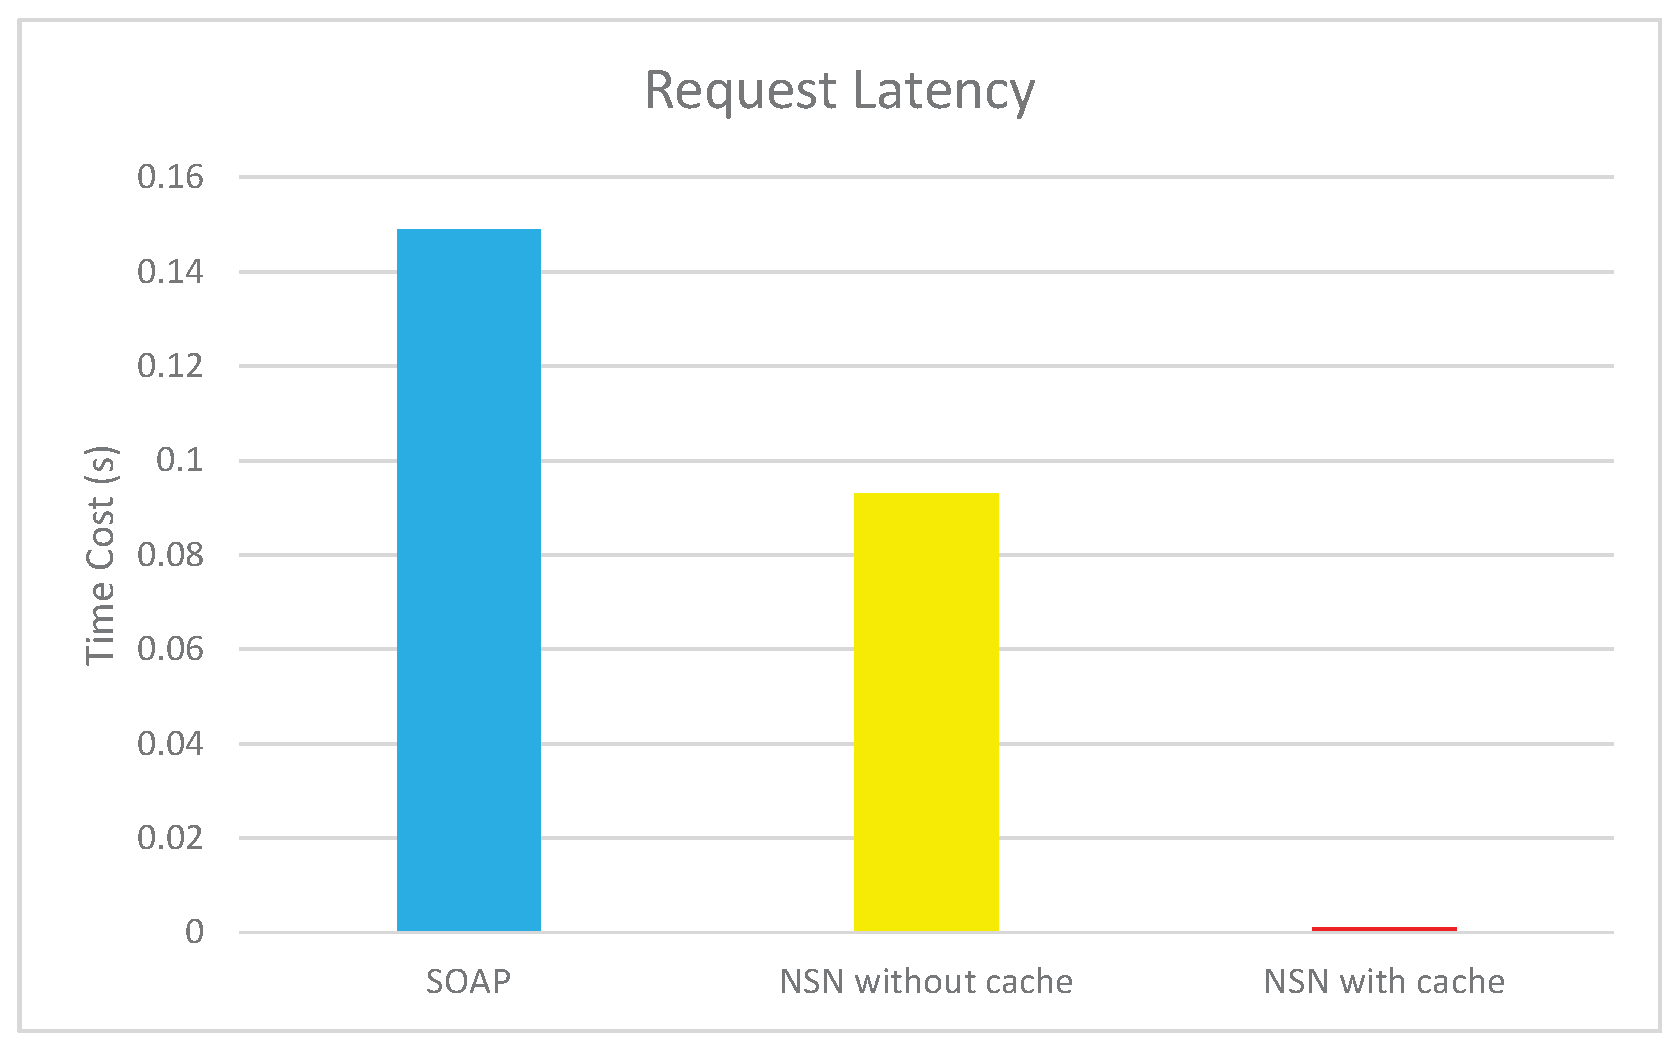
\includegraphics[width=0.7\textwidth]{cache-2}
  \caption{NSN缓存对传输速度的影响}
  \label{fig:cache-2}
\end{figure}

\subsection{服务迁移}
NSN的一个重要特性是将服务的名字与服务的具体位置解耦,服务可以不仅仅限制在同一台主机上。同时由于NSN的安全属性,同名服务还可以在多台主机上同时分布。在云计算服务中,虚拟机或者服务进程迁移在负载均衡以及服务弹性配置中是一项重要功能。本实验评估了服务从一台主机迁移到另一台主机的时候对服务的影响。实验环境为同一数据中心网络的两个子网。客户端在向一台主机不断地请求服务。在10s时服务在一台主机上关闭的同时,在另一台机器上启动。图\ref{fig:migration}表示在实验过程中,客户端发送的请求被响应的情况。可以看到在0.2秒内服务得到恢复。

\begin{figure}[H]
  \centering
  \includegraphics[width=0.7\textwidth]{migration}
  \caption{服务迁移对服务请求处理的影响}
  \label{fig:migration}
\end{figure}

\subsection{服务可用性}
在分布式的服务网络中,服务的可用性也是一项重要的服务评价指标。在本实验中,在N. Virginia的不同子网中部署了四台相同提供相同服务的主机,即服务名字前缀相同。在Oregon数据中心中恒定发送每秒200次服务请求。服务端在0s中启动两台1,2号服务主机,10s时3号服务主机,20s时启动4号服务主机,30是时关闭1号服务主机,40是时关闭2号服务主机,50s时关闭3,4号服务至极服务主机。在图\ref{fig:avail-2}中,可以看到服务请求与服务处理速度基本相等,在40s附近有非常短暂的服务中断。分布式系统中单独服务的频繁启动关闭对于服务可用性的影响很小。

\begin{figure}[H]
  \centering
  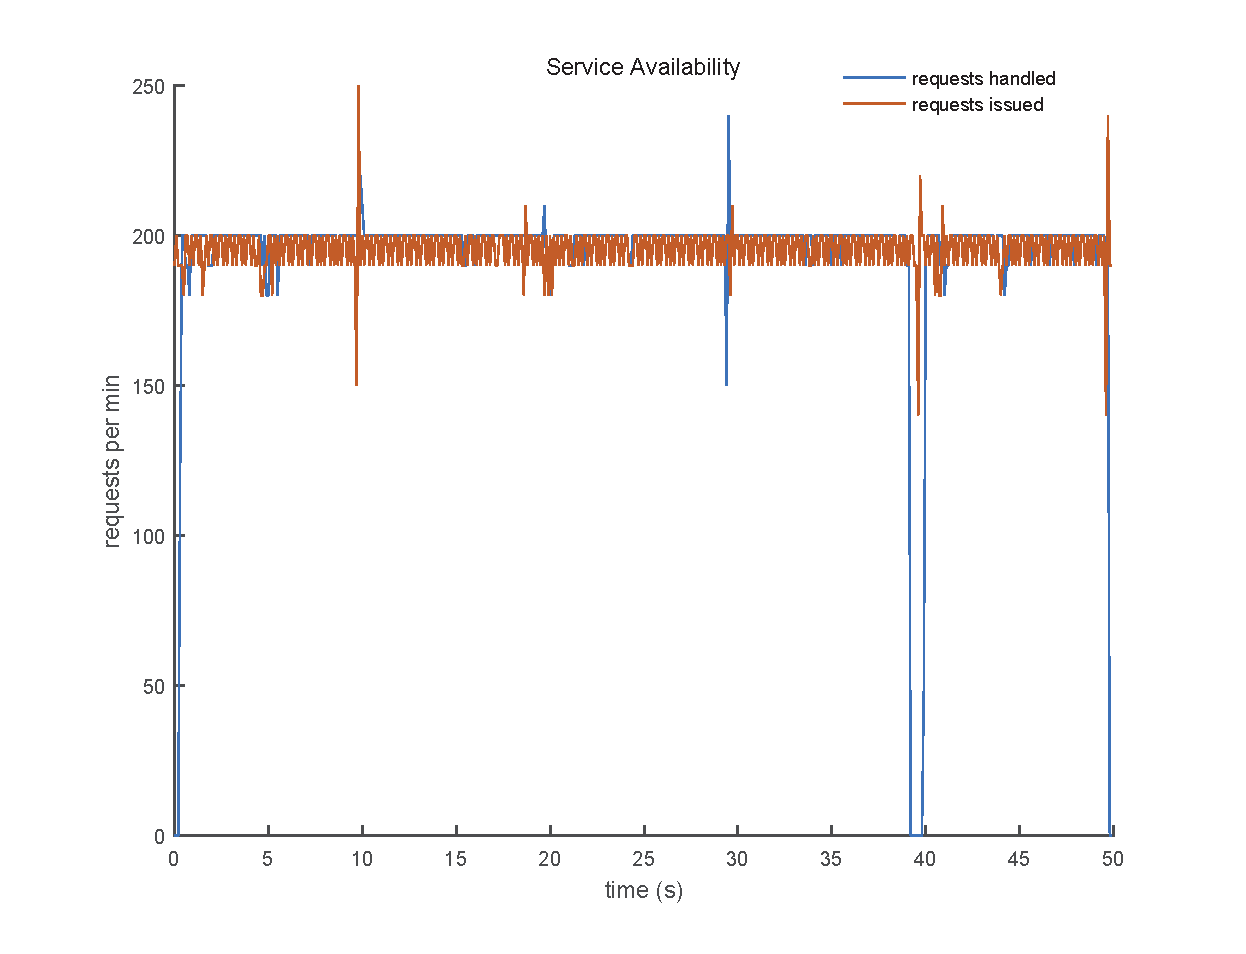
\includegraphics[width=0.7\textwidth]{avail-2}
  \caption{服务可用性测试}
  \label{fig:avail-2}
\end{figure}

\subsection{服务策略配置}
NSN基于NDN网络进行请求的路由和转发。在NDN网络中,可以配置请求转发策略。在本实验中配置了两种转发策略,best-route和随机转发策略。best-route为NDN的默认转发策略,即转发给最近转发请求中,平均延时最小的一个端口。rondom策略为随即平均地转发给任意一个端口。图\ref{fig:strategy:best-route}中表示为在best-route策略下,两台相同服务的主机响应请求的情况。可以看到当网络服务质量比较好时,始终转发到同一个服务主机。图\ref{fig:strategy:random}中表示随机转发策略下两台主机的服务处理情况,可以看到服务响应速率基本一致。

\begin{figure}[H]
\begin{minipage}[t]{0.5\linewidth}
\centering
\includegraphics[width=2.5in]{best-route}
\caption{best-route策略双host请求处理分布}
\label{fig:strategy:best-route}
\end{minipage}%
\begin{minipage}[t]{0.5\linewidth}
\centering
\includegraphics[width=2.5in]{random}
\caption{random策略双host请求处理分布}
\label{fig:strategy:random}
\end{minipage}
\end{figure}

\subsection{服务扩展性}
服务扩展性指的是,服务性能可以随服务主机的增加线性扩展。在本实验中,N. Virginia的不同子网中运行四台服务,服务转发采用random策略,同时客户端以比较大的速率发送服务请求。在0s时启动两台服务主机,并在10s时再启动两台主机。图\ref{fig:scale}表示的是四台服务主机处理请求总和的情况。可以看到在小范围内可以实现服务性能的线性扩展。但是服务性能的扩展性同样受制于转发程序的处理效率,网络带宽等因素,本实验只是在前两者性能得到保证情况下的性能可扩展。

\begin{figure}[H]
  \centering
  \includegraphics[width=0.7\textwidth]{scale}
  \caption{服务扩展测试}
  \label{fig:scale}
\end{figure}

\section{综合分析与结论}
